The worked examples provided are intended to further illustrate how to use \bulk to answer specific questions and conduct investigatons. Each example uses a different, publicly available dataset and can be replicated by readers of this manual. 

\subsection {Encoding}
\newcommand\charpicture[1]{\raisebox{-2pt}[0pt][0pt]{\includegraphics[height=11pt]{#1}}}
We describe the encoding system here in order to prepare users to view
the feature files produced by \bulk. Unicode is the international
standard used by all modern computer systems to define a mapping
between information stored inside a computer and the letters, digits,
and symbols that are displayed on the screens or printed on
paper. UTF-8 is a variable width encoding that can represent every
character in the Unicode character set. It was designed for backward
compatibility with ASCII and to avoid the complications of endianness
and byte order marks in UTF-16 and UTF-32. Feature files in \bulk are
all coded in UTF-8 format. This means that the odd looking symbols,
such as accented characters (\`{e} ), funny symbols
(\charpicture{otherPics/U+2234}) and the occasional Chinese
character (\charpicture{otherPics/U+611B}) that may show up in the
files are legitimate. Glyphs from language, for example, Cyrillic
(\charpicture{otherPics/U+0428}) or Arabic (\charpicture{otherPics/U+062D}) may show up in features files as all
foreign languages can be coded in UTF-8 format. It is perfectly
appropriate and typical to open up a feature file and see characters
that the user may not recognize.\\

\section{2009-M57 Patents Scenario}
The 2009-M57-Patents scenario tracks the first four weeks of corporate history of the (fictional) M57 Patents company. The company started operation on Friday, November 13th, 2009, and ceased operation on Saturday, December 12, 2009. This specific scenario was built to be used as a teaching tool both as a disk forensics exercise and as a network forensics exercise. The scenario data is also useful for computer forensics research because the hard drive of each computer and each computers memory were imaged every day. In this example, we are not particularly interested in the exercises related to illegal activity, exfiltration and eavesdropping; they do however provide interesting components for us to examine in the example data\cite{m57scenario}.

\subsection{Run \bulk with the Data}
For this example, we downloaded and utilized one of the disk images from the 2009-M57-Patents Scenario. Those images are available at \url{http://digitalcorpora.org/corp/nps/scenarios/2009-m57-patents/drives-redacted/}. The file used throughout this example is called \texttt{charlie-2009-12-11.E01}. Running \bulk on the command line produces the following output (text input by the user is bold):\\

\begingroup
\footnotesize
\texttt{C:\textbackslash bulk\_extractor\textgreater \textbf{bulk\_extractor -o ../Output/charlie-2009-12-11 charlie-2009-12-11.E01}}
\endgroup
\begingroup
\footnotesize
\begin{Verbatim}[fontfamily=courier, commandchars=\\\{\}]
bulk_extractor version: 1.4.0
Input file: charlie-2009-12-11.E01
Output directory: ../Output/charlie-2009-12-11
Disk Size: 10239860736
Threads: 4
 8:02:08 Offset 67MB (0.66%) Done in  1:21:23 at 09:23:31
 8:02:34 Offset 150MB (1.47%) Done in  1:05:18 at 09:07:52
 8:03:03 Offset 234MB (2.29%) Done in  1:01:39 at 09:04:42
 8:03:49 Offset 318MB (3.11%) Done in  1:09:19 at 09:13:08
...
9:06:23 Offset 10049MB (98.14%) Done in  0:01:13 at 09:07:36
9:06:59 Offset 10133MB (98.96%) Done in  0:00:41 at 09:07:40
9:07:29 Offset 10217MB (99.78%) Done in  0:00:08 at 09:07:37

All data are read; waiting for threads to finish...
Time elapsed waiting for 4 threads to finish:
     (timeout in 60 min .)
Time elapsed waiting for 3 threads to finish:
    7 sec (timeout in 59 min 53 sec.)
Thread 0: Processing 10200547328
Thread 2: Processing 10217324544
Thread 3: Processing 10234101760

Time elapsed waiting for 2 threads to finish:
    13 sec (timeout in 59 min 47 sec.)
Thread 0: Processing 10200547328
Thread 2: Processing 10217324544

All Threads Finished!
Producer time spent waiting: 3645.8 sec.
Average consumer time spent waiting: 3.67321 sec.
*******************************************
** bulk_extractor is probably CPU bound. **
**    Run on a computer with more cores  **
**      to get better performance.       **
*******************************************
Phase 2. Shutting down scanners
Phase 3. Creating Histograms
   ccn histogram...   ccn_track2 histogram...   domain histogram...
   email histogram...   ether histogram...   find histogram...
   ip histogram...   lightgrep histogram...   tcp histogram...
   telephone histogram...   url histogram...   url microsoft-live...
   url services...   url facebook-address...   url facebook-id...
   url searches...Elapsed time: 3991.77 sec.
Overall performance: 2.56524 MBytes/sec
Total email features found: 15277
\end{Verbatim}
\endgroup
\begin{figure}
	\center
	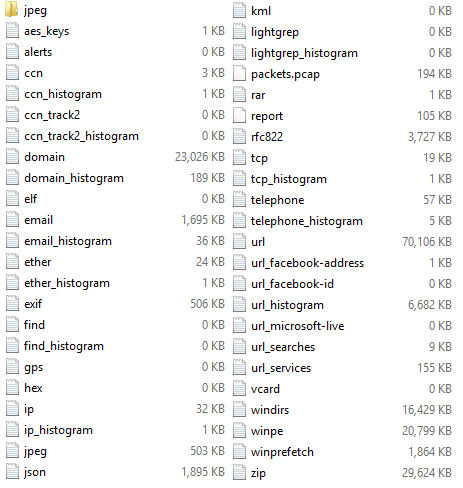
\includegraphics[scale=1.00]{charlieRunOutput.png}
	\caption{Screenshot from Windows Explorer of the Output Directory Created by the \bulk run}
	\label{fig:charlieOutput}
\end{figure}
All of the results from the \bulk run are stored in the output directory \textit{charlie-2009-12-11}. The contents of that directory after the run include the feature files, histogram files and carved output. Figure ~\ref{fig:charlieOutput} is a screenshot of the Windows output directory. Additionally, the following output shows a list of the files, directories and their sizes under Linux:

\begingroup
\footnotesize
\texttt{C:\textbackslash bulk\_extractor\textbackslash charlie-2009-12-11\textgreater \textbf{ls -s -F}}
\endgroup
\begingroup
\footnotesize
\begin{Verbatim}[fontfamily=courier, commandchars=\\\{\}]
    1 aes_keys.txt                  0 kml.txt
    0 alerts.txt                    0 lightgrep.txt
    4 ccn.txt                       0 lightgrep_histogram.txt
    1 ccn_histogram.txt           196 packets.pcap
    0 ccn_track2.txt                1 rar.txt
    0 ccn_track2_histogram.txt    108 report.xml
23028 domain.txt                 3728 rfc822.txt
  192 domain_histogram.txt         20 tcp.txt
    0 elf.txt                       4 tcp_histogram.txt
 1696 email.txt                    60 telephone.txt
   36 email_histogram.txt           8 telephone_histogram.txt
   24 ether.txt                 70108 url.txt
    1 ether_histogram.txt           1 url_facebook-address.txt
  508 exif.txt                      0 url_facebook-id.txt
    0 find.txt                   6684 url_histogram.txt
    0 find_histogram.txt            0 url_microsoft-live.txt
    0 gps.txt                      12 url_searches.txt
    0 hex.txt                     156 url_services.txt
   32 ip.txt                        0 vcard.txt
    4 ip_histogram.txt          16432 windirs.txt
   12 jpeg/                     20800 winpe.txt
  504 jpeg.txt                   1864 winprefetch.txt
 1896 json.txt                  29624 zip.txt
\end{Verbatim}
\endgroup
Many of the feature files and histograms are populated with data. Additionally, there were some JPEG files carved and placed in the \textit{jpeg} directory. In the following sections, we demonstrate how to look at these results to discover more information about the disk user and the files contained on the disk image.

\subsection{Digital Media Triage}
Digital media triage is the process of using the results of a rapid and automated analysis of the media, performed when the media is first encountered to determine if the media is likely to have information of intelligence value and, therefore, should be prioritized for immediate analysis. \bulk performs bulk data analysis to help investigators quickly decide which piece of digital media is the most relevant and useful to an investigation. Thus, \bulk can be used to aid in investigations (through the identification of new leads and social networks) rather than just aiding in conviction-support (through the identification of illegal materials)\cite{digitalmediatriage}.\\

In this example, we look at the \texttt{charlie-2009-12-11.E01} image to quickly assess what kinds of information useful to an investigation might be present on the disk. For the purposes of this example, we will assume we are investigating corporate fraud and trying to discover the answers to the following questions:
\begin{itemize}
\item Who are the users of the drive?
\item Who is this person communicating with?
\item What kinds of websites have they have been visiting most often?
\item What search terms are used?
\end{itemize}

To answer many of these questions, we look at the identify information on the drive including email addresses, credit card information, search terms, Facebook IDs, domain names and vCard data. The output files created by \bulk contain all of this type of information that was found on the disk image. \\

The scenario setup leads us to believe that Charlie is the user of the this drive (based on the name of the disk image). First, we look at \texttt{email.txt} to find information about the email addresses contained on the disk. The first two lines of the email features found are the following (each block of text represents one long line of offset, feature and context):
\lstset{style=customfile}
\begin{lstlisting}
50395384	n\x00o\x00m\x00b\x00r\x00e\x00_\x001\x002\x003\x00@\x00h\x00o\x00t
\x00m\x00a\x00i\x00l\x00.\x00c\x00o\x00m\x00    e\x00m\x00p\x00l\x00o\x00\x00\x0A\x00
\x09\x00n\x00o\x00m\x00b\x00r\x00e\x00_\x001\x002\x003\x00@\x00h\x00o\x00t\x00m
\x00a\x00i\x00l\x00.\x00c\x00o\x00m\x00\x0A\x00\x09\x00m\x00i\x00n\x00o\x00m\x00b\x00

50395432	m\x00i\x00n\x00o\x00m\x00b\x00r\x00e\x00@\x00m\x00s\x00n\x00.\x00c
\x00o\x00m\x00	i\x00l\x00.\x00c\x00o\x00m\x00\x0A\x00\x09\x00m\x00i\x00n\x00o\x00m
\x00b \x00r\x00e\x00@\x00m\x00s\x00n\x00.\x00c\x00o\x00m\x00\x0A\x00\x09\x00e\x00j
\x00e\x00m\x00p\x00l\x00
\end{lstlisting}

It is important to note that UTF-16 formatted text is escaped with \textbackslash x00. This means that "\textbackslash x00t \textbackslash x00e \textbackslash x00x \textbackslash x00t" translates to "text." The first two features found are "nombre\_123@hotmail.com" and "minombre@msn.com."  Both of the offset values, 50395384 and 50395432, are early on the disk. At this point, there is no way to know if either of these email addresses are of any significance unless they happen to belong to a suspect or person related to the investigation. The first set of email features found appear on the disk printed in UTF-16 formatted text, like the lines above.\\

Further down in the feature file, we find the following:
\lstset{style=customfile}
\begin{lstlisting}
9263459	charlie@m57.biz	21)(88=Charlie <charlie@m57.biz>)(89\x0D\x0A    =Pat 
9263497	pat@m57.biz	    =Pat McGoo <pat@m57.biz>)(8B=WELCOME TO
\end{lstlisting}

Finding Charlie's email address on the computer begins to further confirm the assumption that this is his computer. The \texttt{email\_histogram.txt} file provides important information. It shows the most frequently occurring email addresses found on the disk. The following is an excerpt from that top of that file:
\lstset{style=customfile}
\begin{lstlisting}
n=875	mozilla@kewis.ch	(utf16=3)
n=651	charlie@m57.biz	(utf16=120)
n=605	ajbanck@planet.nl
n=411	mikep@oeone.com
n=395	belhaire@ief.u-psud.fr
n=379	premium-server@thawte.com	(utf16=11)
n=356	lilmatt@mozilla.com
n=312	cedric.corazza@wanadoo.fr
\end{lstlisting}
This histogram output shows us that Charlie's email address is the second most frequently occurring name on the disk. It would likely be the first but, as described in the scenario description, this company has only been in business for three weeks and its employees are new users of the computers. Looking at this histogram file also gives us some insight into who the user of this disk is communicating with. Those email addresses occurring most frequently that are not part of the software installed on the machine (such as ajbanck@planet.nl) might indicate addresses of people with whom the drive user is corresponding or they may result from other software or web pages that were downloaded. (In this case, the email is from a Firefox extension.)\\

The file \texttt{domain.txt} provides a list of all the "domains" and host names that were found. The sources include URLS, email and dotted quads. Much of the beginning of the feature file is populated with microsoft.com domains. This is largely due to the fact that the disk image is from a Windows machine. Further down in the file we find the following:
\lstset{style=customfile}
\begin{lstlisting}
53878576	www.uspto.gov	<a href="http://www.uspto.gov/patft/index.htm
53879083	www.uspto.gov	<A HREF="http://www.uspto.gov/patft/help/help
53880076	ebiz1.uspto.gov	<A HREF="http://ebiz1.uspto.gov/vision-service/
53880536	ebiz1.uspto.gov	<A HREF="http://ebiz1.uspto.gov/vision-service/
\end{lstlisting}

The domains that were found make sense given that the disk image was obtained from a startup company that deals with patents. Many of the domains found in the file are also in UTF-16 format (with "escaped" characters). It is also worth noting as users browse the domain output file that domains are common in compressed data.\\

The \texttt{domain\_histogram.txt} file provides a histogram of the domains found on the disk image. It tends to give us better information for digital media triage than the \texttt{domain.txt} file as it provides information about which domains most frequently appear on the disk image and not just the order in which they were found. The beginning of the histogram file looks like the following:
\lstset{style=customfile}
\begin{lstlisting}
n=10749	www.w3.org
n=6670	chroniclingamerica.loc.gov
n=6384	openoffice.org
n=5998	www.uspto.gov
n=5733	www.mozilla.org
n=5212	www.osti.gov
n=4952	www.microsoft.com
n=4470	patft.uspto.gov
\end{lstlisting}

Many of these domains are part of the operating system, such as openoffice.org, but some are not, such as www.uspto.gov. The histogram file provides insight into the users activity on the machine and which sites they were most frequently visiting. \\

The file \texttt{rfc822.txt} primarily provides email headers and HTTP headers both of which are in a format specified by RFC822, the Internet Message Standard. It can be useful to see the subject of emails that have been sent and information form HTTP requests. The following is an excerpt from the text file:
\lstset{style=customfile}
\begin{lstlisting}
114074196 SUBJECT:softabs	ll|micro)\x5CW?cap\x00SUBJECT:softabs\x00SUBJECT:Caili
114074212 SUBJECT:Cailis	SUBJECT:softabs\x00SUBJECT:Cailis\x00\x00SUBJECT:st0ck
114074228 SUBJECT:st0ck	SUBJECT:Cailis\x00\x00SUBJECT:st0ck\x00\x00\x00SUBJECT:Your 
114074244 SUBJECT:Your Personal Quarantine Folder
SUBJECT:st0ck\x00\x00\x00SUBJECT:Your Personal Quarantine Folder\x00SUBJECT:rolex\x00
114074284	SUBJECT:rolex arantine Folder\x00SUBJECT:rolex\x00\x00\x00SUBJECT:(bro
\end{lstlisting}
Much of what is found in the file shown above are spam messages.\\

Telephone numbers found on the disk image are stored in \texttt{telephone.txt}. This following numbers found in the file are clearly for technical support (found within installed software):
\lstset{style=customfile}
\begin{lstlisting}
88850883 (800) 563-9048 rmation centre: (800) 563-9048\x0D\x0A<BR><b><i>Tech
88850995 (905) 568-4494 indows&nbsp;95: (905) 568-4494\x0D\x0A<BR> Microsoft
88851056 (905) 568-2294 ice components: (905) 568-2294\x0D\x0A<BR> Other sta
88851111 (905) 568-3503 hnical support: (905) 568-3503\x0D\x0A<BR> Priority 
88851162 (800) 668-7975 rt information: (800) 668-7975\x0D\x0A<BR> Text Tele
\end{lstlisting}
The next set of "telephone" numbers are clearly bogus numbers:
\lstset{style=customfile}
\begin{lstlisting}
3649684174 008-017-0108 WA,98366,1,4031-008-017-0108,City of Port Or
3649684741 000-031-0009 98337,0.13,3768-000-031-0009,Kitsap County C
3649818237 000-001-0005 8312,2.25,"3768-000-001-0005, 3768-000-003-0
3649818274 000-004-0002 0-003-003, 3768-000-004-0002, 3768-000-005-0
\end{lstlisting}
Finally, many of the numbers found are legitimate ones. These numbers were all found in GZIP compressed data:
\lstset{style=customfile}
\begin{lstlisting}
3772517888-GZIP-28322 (831) 373-5555 onterey - <nobr>(831) 373-5555</nobr><br><a cl
3772517888-GZIP-29518 (831) 899-8300 Seaside - <nobr>(831) 899-8300</nobr><br><a cl
3772517888-GZIP-31176 (831) 899-8300 Seaside - <nobr>(831) 899-8300</nobr><br><a cl
\end{lstlisting}
Typically, the file \texttt{telephone\_histogram.txt} is the best place to look for phone numbers. In this file, the non-digits are extracted from the phone numbers. The following is an excerpt from the beginning of that file:
\lstset{style=customfile}
\begin{lstlisting}
n=42	+14159618830
n=35	8477180400
n=24	+27112570000
n=24	2225552222
n=18	8005043248
n=15	2225551111
n=13	8662347350
n=12	8772768437
n=11	2522277013
\end{lstlisting}
Investigators looking for specific information about the user of a disk image or who they have been communicating with can look quickly at this file and see how frequently numbers appear. It also consolidates the numbers in a way that makes it easy for investigators looking for a specific number or set of numbers to see them quickly.\\

Finally, in performing digital media triage on the disk image, investigators would like to know what specific URLs have been visited and what search terms the user has been using. The set of URL files provided as output provide insight into this information. First, \texttt{url.txt} contains the URLs found on the disk. The following is an excerpt from that file (note that the UTF-16 formatted information is escaped):
\lstset{style=customfile}
\begin{lstlisting} 
175165385 http://www.unicode.org/reports/tr25/#_TocDelimiters E and U+23DF:\x0A#
http://www.unicode.org/reports/tr25/#_TocDelimiters\x0A\x5Cu23DE = \x5CuE13B

159045397 h\x00t\x00t\x00p\x00:\x00/\x00/\x00w\x00w\x00w\x00.\x00d\x00o\x00w
\x00n\x00l\x00o\x00a\x00d\x00.\x00w\x00i\x00n\x00d\x00o\x00w\x00s\x00u\x00p
\x00d\x00a\x00t\x00e\x00.\x00c\x00o\x00m\x00/\x00m\x00s\x00d\x00o\x00w\x00n\x00l\x00o
\x00a\x00d\x00/\x00u\x00p\x00d\x00a\x00t\x00e\x00/\x00s\x00o\x00f\x00t\x00w\x00a\x00r
\x00e\x00/\x00s\x00e\x00c\x00u\x00/\x002\x000\x000\x008\x00/\x000\x006\x00/\x00w\x00i
\x00n\x00d\x00o\x00w\x00s\x00x\x00p\x00-\x00k\x00b\x009\x005\x001\x003\x007\x006\x00-
\x00v\x002\x00-\x00x\x008\x006\x00-\x00e\x00n\x00u\x00_\x00e\x009\x00b\x006\x008\x00c
\x005\x00e\x006\x003\x00a\x00c\x00b\x005\x007\x008\x006\x00a\x000\x005\x00b\x005\x003
\x00b\x004\x00 \xB4\xF4\x82\x94C\xE3\xB6C\xB1p\x9Ae\xBC\x82,wh\x00t\x00t\x00p\x00:
\x00/\x00/\x00w\x00w\x00w\x00.\x00d\x00o\x00w\x00n\x00l\x00o\x00a\x00d\x00.\x00w
\x00i\x00n\x00d\x00o\x00w\x00s\x00u\x00p\x00d\x00a\x00t\x00e\x00.\x00c\x00o
\x00m\x00/\x00m\x00s\x00d\x00o\x00w\x00n\x00l\x00o\x00a\x00d\x00/\x00u\x00p\x00d
\x00a\x00t\x00e\x00/\x00s\x00o\x00f\x00t\x00w\x00a\x00r\x00e\x00/\x00s\x00e\x00c\x00u
\x00/\x002\x000\x000\x008\x00/\x000\x006\x00/\x00w\x00i\x00n\x00d\x00o\x00w\x00s\x00x
\x00p\x00-\x00k\x00b\x009\x005\x001\x003\x007\x006\x00-\x00v\x002\x00-\x00x\x008\x006
\x00-\x00e\x00n\x00u\x00_\x00e\x009\x00b\x006\x008\x00c\x005\x00e\x006\x003\x00a\x00c
\x00b\x005\x007\x008\x006\x00a\x000\x005\x00b\x005\x003\x00b\x004\x003\x003\x002\x004
\x006\x005\x00d\x00e\x00

175197993	http://www.uspto.gov/patft/index.html enter>\x0A<a href="http://www.
uspto.gov/patft/index.html"><img src="/net

175198500	http://www.uspto.gov/patft/help/help.htm e></a>\x0A<AHREF="http://www.
uspto.gov/patft/help/help.htm"><IMG BORDER="0
\end{lstlisting}
The file \texttt{url\_histogram.txt} provides the histogram of the potential urls. In that file, UTF-16 formatted text is converted to UTF-8. Note that not all URLs contained in the histogram file are accurate. The are actually URLs that were typed into a web browser. The following are lines taken from that file:
\lstset{style=customfile}
\begin{lstlisting}
n=3922	http://www.mozilla.org/keymaster/gatekeeper/there.is.only.xul	(utf16=2609)
n=859	http://www.mozilla.org/keymaster/gatekeeper/there.is.only.xu	(utf16=858)
...
n=2	http://math.nist.gov/~KRemington/papers/europvm.ps
n=2	http://math.nist.gov/~MDonahue/pubs/nan.ps.gz
n=2	http://math.nist.gov/~RBoisvert/publications/ADL95.ps.gz
n=2	http://math.nist.gov/~RBoisvert/publications/IMACS97.ps.gz
\end{lstlisting}
Because the histogram file converts the UT-16 formatted text to UTF-8, the histogram file is more human readable than the \texttt{url.txt} file alone. The files \texttt{url\_facebook.txt}, \texttt{url\_microsoft-live}, \texttt{url\_services} and \texttt{url\_searches} all extract specific types of information from URLs. The most useful for digital media triage is likely the file \texttt{url\_searches.txt} because it shows histogram of searches from the disk image. Searches frequently convey intent. The following is an excerpt from that file:
\lstset{style=customfile}
\begin{lstlisting}
n=60	1
n=53	exotic+car+dealer
n=41	ford+car+dealer
n=34	2009+Shelby
n=25	steganography
n=23	General+Electric
n=23	time+travel
n=19	steganography+tool+free
n=19	vacation+packages
n=16	firefox
n=16	quicktime
n=14	7zip
\end{lstlisting}


The file \texttt{ccn.txt} provides credit card numbers that have been found on the disk. Based on the scenario set-up for this disk image, credit card numbers are not necessarily highly relevant to this investigation. However, \bulk did find some credit card numbers on this disk image that are not actually credit card numbers; This is common behavior so it is worth examining the file here to demonstrate how it can be used in other investigations. The credit card number finder considers a pattern of digits and uses the Luhn checksum algorithm and the distribution of digits and the local context to identify potential credit card numbers. It is important to note that there are frequently false positives. The first few lines of the \texttt{ccn.txt} file for this disk image look like the following:
\lstset{style=customfile}
\begin{lstlisting}
88284672-GZIP-177427 5273347458642687 734B55CD5\x0A5273347458642687\x0AC0841BAFA1B4C28
4814857216-GZIP-793 4015751530102097 ebO.d=0;ebO.rnd=4015751530102097;ebO.title="";eb
4909069775 6543210123456788	\x0Addadd7540 add '6543210123456788' 0.499999999   
4909069811 6543210123456788 499999999   -> '6543210123456788' Inexact Rounde
4909069861 6543210123456788 \x0Addadd7541 add '6543210123456788' 0.5           
4909069897 6543210123456788 5           -> '6543210123456788' Inexact Rounde
4909069947 6543210123456788 \x0Addadd7542 add '6543210123456788' 0.500000001   
5304221350 5678901234560000 +4   -> 5678901234560000\x0D\x0Addshi052 shift
5612375618 6543210123456788 \x0D\x0Aaddx6240 add '6543210123456788' 0.499999999   
5612375654 6543210123456788 499999999   -> '6543210123456788' Inexact Rounde
5612375703 6543210123456788 \x0D\x0Aaddx6241 add '6543210123456788' 0.5           
5612375739 6543210123456788 5 -> '6543210123456788' Inexact Rounde
5612375788 6543210123456788 \x0D\x0Aaddx6242 add '6543210123456788' 0.500000001   
5612715901 5700122152274696 div4036 divide  5700122152274696   5700122152251
\end{lstlisting}
In the above example, `525273347458642687' looks like it could be a valid credit card number from the context (\textbackslash x0A is a new line). The number `4015751530102097' looks like a random number in a piece of Java Script. Note that both of those numbers were compressed; the offset indicates they were found in GZIP streams (shown as a number followed by `-GZIP'). The numbers whose context include ``Inexact Rounde'' are actually from Python source code and not credit card numbers at all. Again, the \texttt{ccn.txt} tends to alert on a lot of false positives. \\ 

The \texttt{ccn\_track2.txt} file did not find any information in this disk image but is also useful for credit card fraud and identity theft investigations. It will contain credit card track 2 information found on the disk image.\\

Using the files produced by \bulk described above, an investigator can quickly review a disk image for important information that is relevant to an investigation and find actionable intelligence quickly. 

\subsection{Analyzing Imagery} 
The scenario described in the M57 Patents data is not necessarily relevant to an imagery investigation. However, there is imagery information on the disk. We use that information here to demonstrate how imagery information can be analyzed by an investigator using \bulk.\\

The file in the output directory, \texttt{jpeg.txt}, lists all JPEGs that were found on the disk whether they were carved or not. \bulk was run with default values meaning that only encoded JPEGs were carved. The following excerpt from the JPEG file shows information about JPEGs found on the disk image:
\lstset{style=customfile}
\begin{lstlisting}
54798824	../Output/charlie-2009-12-11/jpeg/54783488.jpg	<fileobject><filename>
../Output/charlie-2009-12-11/jpeg/54783488.jpg</filename><filesize>15336</filesize>
<hashdigest type='md5'>13823ce7c21587d31f6eb4474612e660
</hashdigest></fileobject>
\end{lstlisting}
The JPEG described above was not carved because it was not encoded. However, the first section ``../Output/charlie-2009-12-11/jpeg/54783488.jpg'' shows where the file would be found in the output directories if it had been carved. The next section of information also gives the file size, the hash type (in this case `md5') and the hash value of the file (in this case 13823ce7c21587d31f6eb4474612e660). Note that this may not match the hash value of the file in the original file system as \bulk cannot properly carve fragmented files.\\

Information about encoded JPEGs can also be found in the \texttt{jpeg.txt} file. The following excerpt shows a description of a JPEG found in a GZIP format on the disk:
\lstset{style=customfile}
\begin{lstlisting}
3771686400-GZIP-8332	../Output/charlie-2009-12-11/jpeg/3771686400-GZIP-0.jpg
<fileobject><filename>../Output/charlie-2009-12-11/jpeg/3771686400-GZIP-0.jpg
</filename><filesize>8332</filesize><hashdigest type='md5'>
5b77035c983b04996774370f735ea72a</hashdigest></fileobject>
\end{lstlisting}
The JPEG described above was carved and can be found in the \textit{/jpeg} output directory in the file named \texttt{3771686400-GZIP-0.jpg}. The file also gives information about the filesize, hash type and hash ID. That file is shown in the  directory output shown below along with all of the encoded JPEGs that were found on the disk image and were carved. The contents of the \textit{/jpeg} directory are as follows:

\begingroup
\footnotesize
\begin{Verbatim} 
10037939712-GZIP-0.jpg  5324841013-ZIP-0.jpg
10117679783-ZIP-0.jpg   6039195136-GZIP-0.jpg
3761630720-GZIP-0.jpg   6039215616-GZIP-0.jpg
3764534784-GZIP-0.jpg   6039223808-GZIP-0.jpg
3771686400-GZIP-0.jpg   6039232000-GZIP-0.jpg
3771706880-GZIP-0.jpg   6039244288-GZIP-0.jpg
3771715072-GZIP-0.jpg   6039301632-GZIP-0.jpg
3771723264-GZIP-0.jpg   6039318016-GZIP-0.jpg
3771735552-GZIP-0.jpg   6883925636-ZIP-0.jpg
3771792896-GZIP-0.jpg   6884040324-ZIP-0.jpg
3771809280-GZIP-0.jpg   6884056948-ZIP-0.jpg
3771833856-GZIP-0.jpg   7276064256-GZIP-0.jpg
3771858432-GZIP-0.jpg   7279128576-GZIP-0.jpg
429788672-GZIP-0.jpg    8877243047-ZIP-0.jpg
5310405287-ZIP-0.jpg    9948655104-GZIP-0.jpg
\end{Verbatim}
\endgroup
All of these JPEG files can be viewed and used by investigators. The filename is the forensic path of where the JPEG was found. The file \texttt{3771686400-GZIP-0.jpg} mentioned above is shown in Figure ~\ref{fig:carvedJPEG}.

\begin{figure}
	\center
	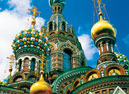
\includegraphics[scale=.90]{carvedJPEG.jpg}
	\caption{A JPEG carved from encoded data on the M57 Patents disk image}
	\label{fig:carvedJPEG}
\end{figure}

\subsection{Password Cracking}
The \textbf{\textit{wordlist}} generates a list of all the words found on the disk that are between 6 and 14 characters long. The word list that is generated by the scanner can be very useful in determining combinations of words to use for password cracking. The scanner is enabled by default because it slows down the \bulk run significantly.  To show the word list in this example, \bulk was run again on the M57 Patents scenario data with the \textbf{\textit{wordlist}} scanner enabled. Running \bulk on the command line with it enabled produces the following output:


\begingroup
\footnotesize
\texttt{C:\textbackslash be\textbackslash \textgreater \textbf{bulk\_extractor -e wordlist -o ../Output/charlie-wordlist charlie-2009-12-11.E01}}
\endgroup
\begingroup
\footnotesize
\begin{Verbatim}[fontfamily=courier, commandchars=\\\{\}]
bulk_extractor version: 1.4.0
Input file: charlie-2009-12-11.E01
Output directory: ../Output/charlie-wordlist
Disk Size: 10239860736
Threads: 4
12:58:46 Offset 67MB (0.66%) Done in  1:14:55 at 14:13:41
...
14:03:24 Offset 10217MB (99.78%) Done in  0:00:08 at 14:03:32
All data are read; waiting for threads to finish...
Time elapsed waiting for 4 threads to finish:
     (timeout in 60 min .)
Time elapsed waiting for 4 threads to finish:
    8 sec (timeout in 59 min 52 sec.)
Thread 0: Processing 10200547328
Thread 1: Processing 10234101760
Thread 2: Processing 10183770112
Thread 3: Processing 10217324544

Time elapsed waiting for 1 thread to finish:
    14 sec (timeout in 59 min 46 sec.)
Thread 3: Processing 10217324544

All Threads Finished!
Producer time spent waiting: 3627.92 sec.
Average consumer time spent waiting: 4.1518 sec.
*******************************************
** bulk_extractor is probably CPU bound. **
**    Run on a computer with more cores  **
**      to get better performance.       **
*******************************************
Phase 2. Shutting down scanners
Phase 3. Uniquifying and recombining wordlist
Phase 3. Creating Histograms
   ccn histogram...   ccn_track2 histogram...   domain histogram...
   email histogram...   ether histogram...   find histogram...
   ip histogram...   lightgrep histogram...   tcp histogram...
   telephone histogram...   url histogram...   url microsoft-live...
   url services...   url facebook-address...   url facebook-id
   url searches...Elapsed time: 4065.09 sec.
Overall performance: 2.51898 MBytes/sec
Total email features found: 152775
\end{Verbatim}
\endgroup

Note that it took 3991.71 seconds to run \bulk without the \textbf{\textit{wordlist}} scanner enabled and, in this case, it took 4065.09 seconds with \textbf{\textit{wordlist}} enabled.  The new output directory contains a file called \texttt{wordlist.txt}. That file has both filenames and words in it. The following is an excerpt from that file:
\lstset{style=customfile}
\begin{lstlisting}
50497556	usemodem.jpg
50497624	usemsn.jpg
50497692	usemsnnow.jpg
50497760	welcome.htm
50497828	whereNow.htm
50497896	xmlutil.js
50497987	^Photoshop
50498009	Resolution
50498050	Global
50498057	Lighting
50498090	Global
50498097	Altitude
50498153	Copyright
50498181	Japanese
50498229	Halftone
50498238	Settings
50498335	Transfer
\end{lstlisting}
The wordlist contains ALL words found on the disk between 6 and 14 characters long. Automated programs can be used to generate passwords from combinations of these words. The \textbf{\textit{wordlist}} scanner also generates a split wordlist containing the same words found in the \texttt{wordlist.txt} file with all words deduplicated, sorted by size and alphabetized. The following is an excerpt from the file \texttt{wordlist\_split\_000.txt} generated from the disk image:
\lstset{style=customfile}
\begin{lstlisting}!!!!!!
concluded|1
concluder/2
concluder/M
concluir/XQ
conclurai/x
conclusion,
conclusion.
conclusione
conclusions
conclusive,
\end{lstlisting}
The split wordlist is the file that is typically fed to password cracking software.

\subsection{Post Processing}
The programs \textbf{identify\_filenames.py} and \textbf{bulk\_diff.py} can provide further insight into the data contained on the disk image. The \textbf{identify\_filenames.py} program can be used on the feature files produced from the \bulk run to show the file location of the features that were found. Running the program on all of the feature files produced by the \bulk run produces the following output (where \textit{charlie-2009-12-11} is the \bulk output directory and \textit{charlieAnnotatedOutput} is where all the annotated files are written):\\

\begingroup
\footnotesize
\texttt{C:\textbackslash be\textbackslash \textgreater \textbf{identify\_filenames.py --all charlie-2009-12-11 charlieAnnotatedOutput}}
\endgroup
\begingroup
\footnotesize
\begin{Verbatim}[fontfamily=courier, commandchars=\\\{\}]
Reading file map by running fiwalk on charlie-2009-12-11.E01
Processed 1000 fileobjects in DFXML file
Processed 2000 fileobjects in DFXML file
...
Processed 39000 fileobjects in DFXML file
Processed 40000 fileobjects in DFXML file
feature_file: aes_keys.txt
feature_file: ccn.txt
feature_file: domain.txt
feature_file: email.txt
feature_file: ether.txt
feature_file: exif.txt
feature_file: ip.txt
feature_file: jpeg.txt
feature_file: json.txt
feature_file: rar.txt
feature_file: rfc822.txt
feature_file: telephone.txt
feature_file: url.txt
feature_file: windirs.txt
feature_file: winpe.txt
feature_file: winprefetch.txt
feature_file: zip.txt
******************************
** Total Features:   754038 **
** Total Located:   754038 **
******************************
\end{Verbatim}
\endgroup

Note, in this example that \textbf{fiwalk} is installed on the computer running the \textbf{identify\_filenames.py} program. The directory \textit{charlieAnnotatedOutput} contains all of the annotated feature files, showing the file location of the features. The directory contents are as follows:

\begingroup
\footnotesize
\begin{Verbatim} 
annotated_aes_keys.txt        annotated_rar.txt
annotated_ccn.txt        annotated_rfc822.txt
annotated_domain.txt        annotated_telephone.txt
annotated_email.txt        annotated_url.txt
annotated_ether.txt        annotated_windirs.txt
annotated_exif.txt        annotated_winpe.txt
annotated_ip.txt        annotated_winprefetch.txt
annotated_jpeg.txt        annotated_zip.txt
annotated_json.txt
\end{Verbatim}
\endgroup

The annotated files display the feature with the file in which the feature was found (where it was identified by the program). The following is an excerpt from the \texttt{annotated\_email.txt} file:
\lstset{style=customfile}
\begin{lstlisting}
27767966 pat@m57.biz	m: "Pat McGoo" <pat@m57.biz>\x0D\x0ATo: <charlie@ Documents 
and Settings/Charlie/Application Data/Thunderbird/Profiles/4zy34x9h.default/Mail/Local 
Folders/Inbox dcb794e350bd198c4279614eae6c8b76

27767985 charlie@m57.biz @m57.biz>\x0D\x0ATo: <charlie@m57.biz>,\x0D\x0A\x09<jo@m
57.biz	Documents and Settings/Charlie/Application Data/Thunderbird/Profiles/4zy34x9h.
default/Mail/Local Folders/Inbox dcb794e350bd198c4279614eae6c8b76

27768022 terry@m57.biz jo@m57.biz>,\x0D\x0A\x09<terry@m57.biz>\x0D\x0AX-ASG-Orig-
Su Documents and Settings/Charlie/Application Data/Thunderbird/Profiles/4zy34x9h.def
ault/Mail/Local Folders/Inbox dcb794e350bd198c4279614eae6c8b76
\end{lstlisting}
The email address "pat@m57biz" was found in the file \texttt{Documents and Settings/Charlie/}\newline\texttt{Application Data/Thunderbird/Profiles/4zy34x9h.default/Mail/Local Folders/Inbox} and investigators can refer to that location on the disk image to view the full text.\\

The program \textbf{bulk\_diff.py} shows the difference between two \bulk runs. In this case, we used a disk image from the same user ("charlie") taken almost a month before the disk image that has been used throughout this example. The disk image we have been using throughout this example is dated December 11, 2009. The older disk image we downloaded for comparison is dated November 17, 2009.  The earlier disk image data is stored in a file named \texttt{charlie-2009-11-17.E01} and can be downloaded from \url{http://digitalcorpora.org/corp/nps/scenarios/2009-m57-patents/drives-redacted/}.\\

After running \bulk using the earlier disk image, we ran the program \textbf{bulk\_diff.py} on the output of that disk image and on the output of the \texttt{charlie-2009-12-11.E01} run. To run, we typed the following, piping the output of the program to a file called \texttt{bulkdiffoutput.txt}:
\begin{Verbatim}[commandchars=\\\{\}]
\verbbf{bulk\_diff.py /charlie-2009-11-17 /charlie-2009-12-11 > bulkdiffoutput.txt}
\end{Verbatim} 
The output shows the features differences on the disk image. The following is an excerpt of that output:
\lstset{style=customfile}
\begin{lstlisting}
domain_histogram.txt:
	#in PRE		#in POST	Value
------------------------------------------------------------------------------------
401	4,470		4,069		patft.uspto.gov
181	3,151		2,970		www.wipo.int
295	3,157		2,862		www.google.com
0	2,537		2,537		l.yimg.com
\end{lstlisting}
The output specifically shows the differences in the histograms between the two runs across all of the histogram files that were created. The excerpt above shows that "charlie" (the disk user) visited the domain "patft.uspto.gov" frequently between the time the two images were recorder. It was found 4,069 more times in the later disk image than in the one taken earlier. It also shows that the domain "l.yimg.com" was not found on the earlier disk image but was found 2,537 times on the later disk image. The results are sorted by the amount of the difference. This means that features that are most different appear first. This can be very helpful because those features generally give the most insight into the disk users activity over that period of time.

\section{NPS DOMEX Users Image}
NPS Test Disk Images are a set of disk images that have been created for testing computer forensic tools. These images are free of non-public Personally Identifiable Information (PII) and are approved for release to the general public. The NPS-created data in the images is public domain and free of any copyright restriction; the images may contain some copyrighted data that was made available by the copyright holder. These copyrights, where known, are noted in the files themselves\cite{npsdiskimages}. \\

The NPS DOMEX users image is a disk image of a Windows XP SP3 system that has two users, domexuser1 and domexuser2, who communicate with a third user (domexuser3) via IM and email.  The data is available for download at \url{http://digitalcorpora.org/corp/nps/drives/nps-2009-domexusers/}. For this example, we use the file \texttt{nps-2009-domexusers.E01} which includes the full system including the Microsoft Windows executables. Running \bulk on the command line produces the following output:\\

\begingroup
\footnotesize
\texttt{C:\textbackslash be\textbackslash \textgreater \textbf{bulk\_extractor -o ../Output/nps-2009-domexusers nps-2009-domexusers.E01}}
\endgroup
\begingroup
\footnotesize
\begin{Verbatim}[fontfamily=courier, commandchars=\\\{\}]
bulk_extractor version: 1.4.0
Input file: nps-2009-domexusers.E01
Output directory: ../Output/nps-2009-domexusers2
Disk Size: 42949672960
Threads: 4
16:50:53 Offset 67MB (0.16%) Done in  4:23:43 at 21:14:36
16:51:19 Offset 150MB (0.35%) Done in  3:58:37 at 20:49:56
...
16:13:12 Offset 42849MB (99.77%) Done in  0:00:11 at 16:13:23
16:13:13 Offset 42932MB (99.96%) Done in  0:00:01 at 16:13:14
All data are read; waiting for threads to finish...
Time elapsed waiting for 3 threads to finish:
     (timeout in 60 min .)
Time elapsed waiting for 1 thread to finish:
    6 sec (timeout in 59 min 54 sec.)
Thread 0: Processing 42932895744

Time elapsed waiting for 1 thread to finish:
    12 sec (timeout in 59 min 48 sec.)
Thread 0: Processing 42932895744

All Threads Finished!
Producer time spent waiting: 4254.07 sec.
Average consumer time spent waiting: 89.309 sec.
*******************************************
** bulk_extractor is probably CPU bound. **
**    Run on a computer with more cores  **
**      to get better performance.       **
*******************************************
Phase 2. Shutting down scanners
Phase 3. Creating Histograms
   ccn histogram...   ccn_track2 histogram...   domain histogram...
   email histogram...   ether histogram...   find histogram...
   ip histogram...   lightgrep histogram...   tcp histogram...
   telephone histogram...   url histogram...   url microsoft-live...
   url services...   url facebook-address...   url facebook-id...
   url searches...Elapsed time: 4846.74 sec.
Overall performance: 8.86156 MBytes/sec
Total email features found: 8774
\end{Verbatim}
\endgroup

All of the results from the \bulk run are stored in the output directory \textit{nps-2009-domex}. The contents of that directory after the run are as follows:

\begingroup
\footnotesize
\begin{Verbatim}
    1 aes_keys.txt                  1 kml.txt
    0 alerts.txt                    0 lightgrep.txt
    1 ccn.txt                       0 lightgrep_histogram.txt
    1 ccn_histogram.txt             4 packets.pcap
    0 ccn_track2.txt                1 rar.txt
    0 ccn_track2_histogram.txt    424 report.xml
 7364 domain.txt                  536 rfc822.txt
   44 domain_histogram.txt          1 tcp.txt
    0 elf.txt                       1 tcp_histogram.txt
 1528 email.txt                    48 telephone.txt
   32 email_histogram.txt           4 telephone_histogram.txt
    1 ether.txt                 51888 url.txt
    1 ether_histogram.txt           0 url_facebook-address.txt
  152 exif.txt                      0 url_facebook-id.txt
    0 find.txt                   1240 url_histogram.txt
    0 find_histogram.txt            0 url_microsoft-live.txt
    0 gps.txt                       4 url_searches.txt
    0 hex.txt                      32 url_services.txt
    4 ip.txt                        0 vcard.txt
    1 ip_histogram.txt          15228 windirs.txt
   20 jpeg/                     26516 winpe.txt
  380 jpeg.txt                   1312 winprefetch.txt
  316 json.txt                   1956 zip.txt
\end{Verbatim} 
\endgroup
For this example, we will focus on the files that are most important to malware investigations and cyber investigations, showing how those files can be interpreted and used by investigators.

\subsection{Malware Investigations}
In a malware investigation, investigators are looking for information about programmatic intrusions. In this example, we examine all files that provide information about executables, Windows directory entries and information downloaded from web-based applications. We recommend that "-e xor" be enabled for malware investigations.\\

The file \texttt{windirs.txt} provides information about FAT32 and NTFS directories. It contains most of the disk entries. The following is an excerpt showing one line from the file:
\lstset{style=customfile}
\begin{lstlisting}
281954816	A0001801.dll	<fileobject
src='mft'><atime>2008-10-21T00:45:51Z</atime><attr_flags>8224</attr_flags>
<crtime>2008-10-21T00:45:51Z</crtime><ctime>2008-10-21T00:45:51Z</ctime>
<filename>A0001801.dll</filename><filesize>1000000000000</filesize><filesize_alloc>
0</filesize_alloc><lsn>123437339</lsn><mtime>2008-10-21T00:45:51Z</mtime>
<nlink>1</nlink><par_ref>12017</par_ref><par_seq>3</par_seq><seq>1</seq>
</fileobject>
\end{lstlisting}
The line from the file gives information about the disk entry \texttt{A0001801.dll}. It provides some data about the file including the file size, file creation time (ctime) and time of last file modification (mtime). It is important to note that the error rate for FAT32 entries is high and those entries should be ignored if the drive is not FAT. \\

For investigations on Windows disk images, such as the \texttt{nps-2009-domexusers}, the file \texttt{winpe.txt} shows Windows executables related to the Windows Preinstallation Environment. These file entries contain very long lines. The following is \textbf{one} line from the file:
\lstset{style=customfile}
\begin{lstlisting}
42753536 87d84154e7789013878c6340a4d2d445 <PE><FileHeader Machine=
"IMAGE_FILE_MACHINE_I386"NumberOfSections="3" TimeDateStamp="1208131815"
 PointerToSymbolTable="0"NumberOfSymbols="0"SizeOfOptionalHeader="224">
<Characteristics><IMAGE_FILE_EXECUTABLE_IMAGE />
<IMAGE_FILE_LINE_NUMS_STRIPPED /><IMAGE_FILE_LOCAL_SYMS_STRIPPED />
<IMAGE_FILE_32BIT_MACHINE/><IMAGE_FILE_DLL /></Characteristics>
</FileHeader><OptionalHeaderStandard Magic="PE32" MajorLinkerVersion="7" 
MinorLinkerVersion="10" SizeOfCode="512" SizeOfInitializedData="1536" 
SizeOfUninitializedData="0" AddressOfEntryPoint="0x1046" BaseOfCode=
"0x1000" /><OptionalHeaderWindows ImageBase="0x6c6c0000" SectionAlignment
="1000" FileAlignment="200"MajorOperatingSystemVersion="5" 
MinorOperatingSystemVersion="1" MajorImageVersion="5" 
MinorImageVersion="1" MajorSubsystemVersion="4" MinorSubsystemVersion="0" 
Win32VersionValue="0" SizeOfImage="4000" SizeOfHeaders="400" CheckSum="
0x7485" SubSystem="" SizeOfStackReserve="40000"SizeOfStackCommit="1000"
SizeOfHeapReserve="100000" SizeOfHeapCommit="1000" LoaderFlags="0"
NumberOfRvaAndSizes="10"><DllCharacteristics>
<IMAGE_DLL_CHARACTERISTICS_NO_SEH /></DllCharacteristics>
</OptionalHeaderWindows><Sections><SectionHeader Name=".text" VirtualSize
="be" VirtualAddress="1000" SizeOfRawData="200" PointerToRawData="400" 
PointerToRelocations="0" PointerToLinenumbers="0" ><Characteristics>
<IMAGE_SCN_CNT_CODE /><IMAGE_SCN_MEM_EXECUTE />
<IMAGE_SCN_MEM_READ /></Characteristics></SectionHeader><SectionHeader 
Name=".rsrc" VirtualSize="400" VirtualAddress="2000" SizeOfRawData="400" 
PointerToRawData="600" PointerToRelocations="0" PointerToLinenumbers="0"
><Characteristics><IMAGE_SCN_CNT_INITIALIZED_DATA />
<IMAGE_SCN_MEM_READ /></Characteristics></SectionHeader>
<SectionHeader Name=".reloc" VirtualSize="8" VirtualAddress="3000" 
SizeOfRawData="200" PointerToRawData="a00" PointerToRelocations="0" 
PointerToLinenumbers="0" ><Characteristics><IMAGE_SCN_CNT_INITIALIZED_DATA />
<IMAGE_SCN_MEM_DISCARDABLE /><IMAGE_SCN_MEM_READ /></Characteristics>
</SectionHeader></Sections></PE>
\end{lstlisting}
The first number is the offset and tells you were to find the file. Most executables are not fragmented. The second is the MD5 has of the first 4k of the file that can be used to deduplicate and look up the file in the hash database. Finally, the bulk of the information is contained in the <PE> XML block that breaks out all of the Windows PE header information. It contains information about the File header, the characteristics of the file, Windows header information and section header information.\\

The file \texttt{winprefetch.txt} contains the information from carved files Windows Prefetch that were discovered anywhere on the drive. \bulk will carve the Prefetch files from unallocated space. This extremely useful because Prefetch files are frequently deleted. A single line in the prefetch output file is also very long. The following is only the beginning of one line from the file:
\lstset{style=customfile}
\begin{lstlisting}
55758336	MSIEXEC.EXE	<prefetch><os>Windows
XP</os><filename>MSIEXEC.EXE</filename><header_size>152</header_size>
<atime>2008-10-30T03:17:27Z</atime><runs>14</runs><filenames>
<file>\x5CDEVICE\x5CHARDDISKVOLUME1\x5CWINDOWS\x5CSYSTEM32\x5CNTDLL.DLL
</file><file>\x5CDEVICE\x5CHARDDISKVOLUME1\x5CWINDOWS\x5CSYSTEM32\x5CKERNEL32.DLL
...
\end{lstlisting}
Printing the line out here would cover almost two pages. It includes a lot of information about the Prefetch file including the name of the executable, the name of the DLLs, the directory of DLLs, the atime, the number of runs, the serial number, and the ctime. The Prefetch file is searchable and useable by investigators searching for EXEs or DLLs related to a malware investigation.\\

JSON is the JavaScript Object Notation (used in Facebook, etc). The file \texttt{json.txt}  provides the offset, JSON and MD5 hash of the JSON information found on the disk image. \bulk is great at finding JSON in compressed streams and HIBER files. The following are a few lines from the JSON file:
\lstset{style=customfile}
\begin{lstlisting}
62836579 {"ask":["Ask"],"delicious":["Del.icio.us"],"digg":["Digg"],"email":["Email"],
"favorites":["Favorites"],"facebook":["Facebook"],"fark":["Fark"],"furl":["Furl"],
"google":["Google"],"live":["Live"],"myspace":["MySpace"],"myweb":["Yahoo MyWeb"
,"yahoo-myweb"],"newsvine":["Newsvine"],"reddit":["Reddit"],"sk*rt":["Sk*rt","skrt"],
"slashdot":["Slashdot"],"stumbleupon":["StumbleUpon","su"],"stylehive":["Stylehive"],
"tailrank":["Tailrank","tailrank2"],"technorati":["Technorati"],"thisnext":
["ThisNext"],"twitter":["Twitter"],"ballhype":["BallHype"],"yardbarker":
["Yardbarker"],"kaboodle":["Kaboodle"],"more":["More ..."]}	
26d3b8c5010f4d39250dab3a1c1b839e

62842797 ["6jb4","3j1d","v1me","gu83","uefc","fq1j","r5l7","ftho","gdq9","717h",
"24b7","d0en","ads7","m9b4","n0lq","42c3","p5mp","7hbi","f0g6","7v98","mv86", 
"d0ns","9a8a","64gg","jogl","cehp","mu2r","6h7h","sntb","94ds","n1fv","3a2i",
"3end","l42s","a9j","q3dj","s150","di3s","3nu5","sk74","e39d","mkvj","482d","kfej",
"nlcv","eroi","m6ee","rvaa","9nis","ef6b","g00q","b4hp","kbpq","bm4l","f7iu",
"e5gb","1sbj","rk0a","ck86","1etp","26sr","fivt","3v95","foqq","vtmj","canb",
"bchv","ku35","q4p9","gdkt","gng8","mdb9","ejjg","27k9","30mf","nene",
"smmm","q204","83ot","6kbr","df1o","1q0j","nh32","ebso","d6t5","f2dp",
"3sqp","i4cs","6k7b","a1pv","ki2l","1f7","d6lv","u7r5","9t0e","5h0l","j8kn",
"7akj","9tj","jmu3","1ir1"]	5a04af7518ad74c497c9e74b7025736e

64044544-GZIP-610 ["Top","Left","Right","Bottom"] 5354ef6838974b1979e49ee379883c56
\end{lstlisting}
Some of the JSON features found, such as the one located at '62836579', are comprised of a lot of information in the notation. Other JSON features are very short, such as the feature located at in the GZIP compressed stream at '64044544-GZIP-610.' All of the lines contain the MD5 hash of the JSON that is used for deduplication.\\

The file \texttt{elf.txt} typically contains information about ELF executables, which is the executable file format for Linux and Android systems. The sample corpus used in this example is from a Windows machine and does not contain any ELF executables.

\subsection{Cyber Investigations}
Cyber investigations cover a wide variety of areas. However, most involve looking for encryption keys, hash values or information about ethernet packets. \bulk finds all of those things on the disk and writes them to different output files. Of note, \bulk also finds information in Base64 encoding and decompresses fragments of Windows Hibernation files. There are not specific files created for that processing; the information found in data with these encodings will be processed by other scanners and stored in the appropriate feature files. The fact that a feature came from encoded data will be indicated in the forensic path. The information contained therein may very well be relevant to cyber investigations.\\

AES encryption implementation system sometimes leaves keys in memory and \bulk finds those keys, usually in RAM, Swap or hibernation files. The keys can sometimes be used to decrypt AES encrypted material. The file \texttt{aes.txt} contains the keys that are found. There was only one AES key found on the \texttt{nps-2009-domexusers} disk image. The following is the line that describes it from the keys file including the offset, key and key size descriptor (AES256):
\lstset{style=customfile}
\begin{lstlisting}
1608580652	28 90 90 5e f7 ce b4 a7 2b 7d d9 45 d8 b0 56 99 97 f4 42 
33 35 f1 54 9a 79 36 e7 1c 94 02 28 78 	AES256
\end{lstlisting}

The file \texttt{hex.txt} contains extracted hexidecimal strings of a special length. The block sizes cotained within it are either 128 or 256 due to the fact that those are the sizes used for encryption keys and hash values. The disk image used in this example does not have any of those and the file is blank.\\

\bulk produces network information including PCAP files, Ethernet addresses, and TCP/IP connections. The files \texttt{ether.txt} and \texttt{ether\_histogram.txt} provide a list of ethernet  addresses from packets and ASCII. These are the addresses found on the disk and located in \texttt{ether.txt}:
\lstset{style=customfile}
\begin{lstlisting}
2435863552	00:0C:29:26:BB:CD	 (ether_dhost) 
2435863552	00:50:56:E0:FE:24	 (ether_shost) 
2435865088	00:0C:29:26:BB:CD	 (ether_dhost) 
2435865088	00:50:56:E0:FE:24	 (ether_shost) 
22637986225	00:80:C7:8F:6C:96	 apter.\x0AExample: 00:80:C7:8F:6C:96\x00\x00
\end{lstlisting}
The file {ether\_histogram.txt} groups these ethernet addresses in a histogram:
\lstset{style=customfile}
\begin{lstlisting}
n=2	00:0C:29:26:BB:CD
n=2	00:50:56:E0:FE:24
n=1	00:80:C7:8F:6C:96
\end{lstlisting}
Packets likely traveled from 00:0C:29:26:BB:CD to 00:50:56:E0:FE:24.  The other usage has Ethernet addresses in UTF-16 format.\\

The file \texttt{ip.txt} contains IP addresses from packet carving, not from dotted quads. The following is an excerpt from that file:
\lstset{style=customfile}
\begin{lstlisting}
2435865102	inet_ntop win32	struct ip L (src) cksum-ok
2435865102	inet_ntop win32	struct ip R (dst) cksum-ok
2805534669	123.12.0.192	sockaddr_in
8694397397	135.5.0.234	sockaddr_in
9047318477	123.12.0.192	sockaddr_in
9446959573	135.5.0.234	sockaddr_in
11295228937	1.70.0.1	sockaddr_in
\end{lstlisting}
The \textit{L} or \textit{R} in the 'struct ip' information indicates Local or Remote. This line also includes the IP checksum is ok. The value could also be listed as "cksum-bad" to indicate it is bad. Bad checksums may indicate a false positive and not a legitimate IP address. Finally, the "sockaddr\_in" indicates the IP address is from a "sockaddr\_in" structure. The file \texttt{ip\_histogram.txt} removes the random noise that is found in the \texttt{ip.txt}. Here is an excerpt from the histogram file:
\lstset{style=customfile}
\begin{lstlisting}
n=5	2.172.0.101
n=4	123.12.0.192
n=4	inet_ntop win32
n=3	135.5.0.234
n=2	209.85.147.109
n=2	65.55.15.242
\end{lstlisting}

The file \texttt{packets.pcap} is a pcap file made from carved packet. To view that file, use any packet analysis tool you like (such as \textbf{tcpdump}). Only packets carved from a PCAP  file will have the correct packet time stamp; others will given a time in 1970.\\

Finally, the file \texttt{tcp.txt} contains details about TCP (and UDP) network flows. It contains more detail than \texttt{ip.txt} but investigators should be careful of false positives, as there are often many in this file. The following are the two lines found in that file:
\lstset{style=customfile}
\begin{lstlisting}
2435863566	inet_ntop win32:80 -> inet_ntop win32:1034 (TCP)	 Size: 1472
2435865102	inet_ntop win32:80 -> inet_ntop win32:1034 (TCP)	 Size: 1252
\end{lstlisting}
The file \texttt{tcp\_histogram.txt} often provides further insight into the tcp information found on the disk image. In this case, it does not because there were only two features found. It is important to note that the histogram file still contains a lot of false positives.

